\section{Introducción}
\subsection{Los ciclones tropicales en México}
\begin{frame}
    \begin{figure}[H]
        \centering
        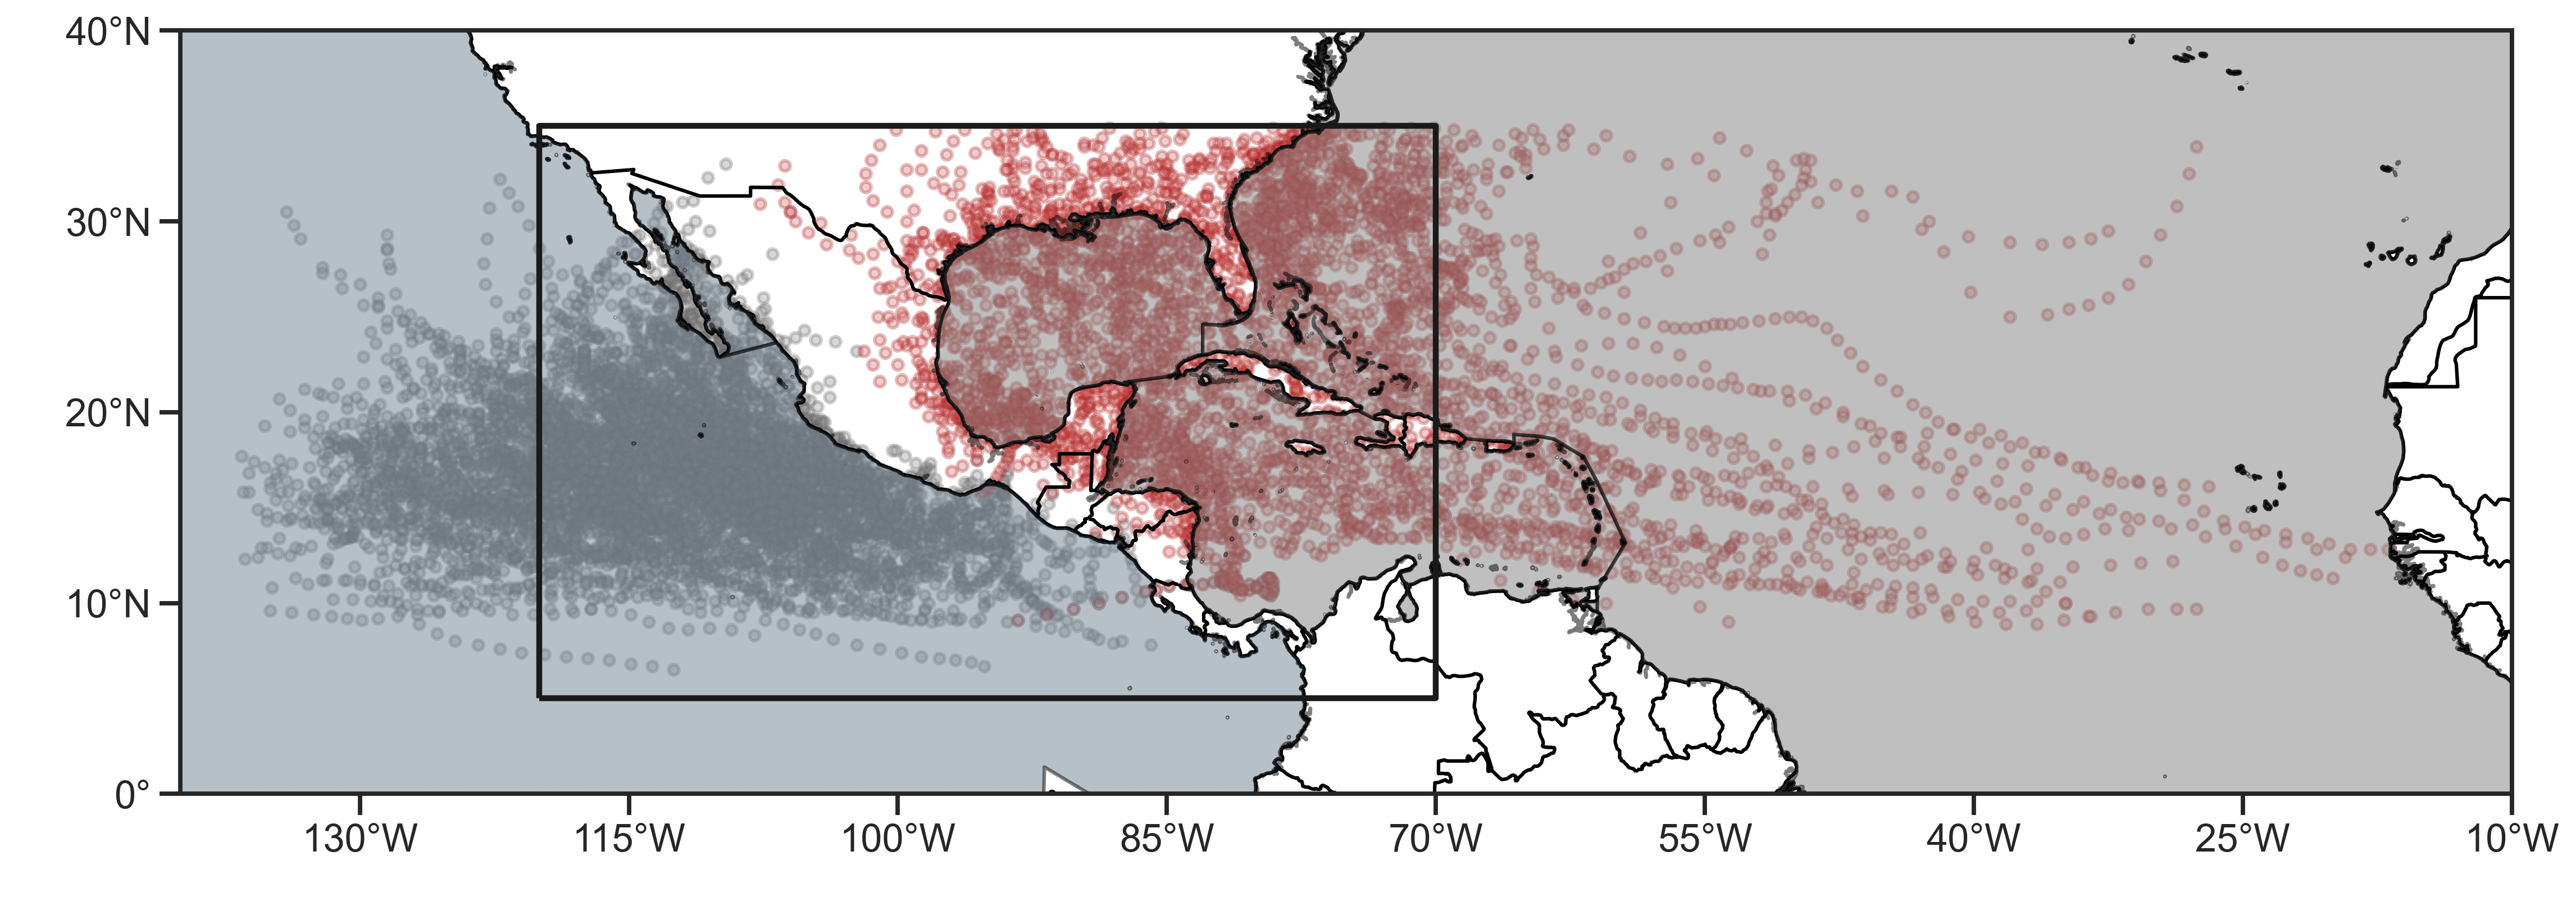
\includegraphics[scale = 0.275]{Images/Figures/Fig_2_1.jpeg}
        \caption{La región de estudio se encuentra marcada por un cuadro negro. Las posiciones de cada 6 horas de los CTs en el Océano Atlántico del norte (NA) y en el Océano Pacífico del este (EP) se encuentran en polígonos rojos y grises, respectivamente}
        \label{fig:fig_1}
    \end{figure}
\end{frame}

\begin{frame}{Escala Saffir-Simpson}
    % Please add the following required packages to your document preamble:

\begin{table}
\centering
\caption{Clasificación de los vientos de los CTs de acuerdo a la escala Saffir-Simpson. Se anexan dos categorías adicionales cuando el CT aún no alcanza la categoría de huracán (Kelman, 2013)}
\label{tab:1.1}
\resizebox{\textwidth}{!}{%
\begin{tabular}{@{}cccc@{}}
\toprule
\multicolumn{2}{c}{\textbf{Categoría}}               & \begin{tabular}[c]{@{}c@{}}\textbf{Vientos Sostenidos} \\ ($km  h^{-1}$)\end{tabular} & \begin{tabular}[c]{@{}c@{}} \textbf{Tipos de daño debido a}\\  \textbf{los vientos del CT}\end{tabular} \\ \midrule
\multicolumn{2}{l}{Depresión Tropical (DT)} & \textless 63                                                           & Daños menores                                                                             \\
\multicolumn{2}{l}{Tormenta Tropical  (TT)}  & 64-118                                                                 & Daños moderados                                                                           \\
\multirow{5}{*}{Huracán}         & 1        & 119-153                                                                & Vientos muy peligrosos                                                                    \\
                                 & 2        & 154-177                                                                & Vientos extremadamente peligrosos                                                         \\
                                 & 3        & 178-208                                                                & Daños devastadores                                                                        \\
                                 & 4        & 209-251                                                                & Daños catastróficos                                                                       \\
                                 & 5        & \textgreater 252                                                       & Daños extraordinarios                                                                     \\ \bottomrule
\end{tabular}%
}
\end{table}
\end{frame}

\begin{frame}
    \begin{figure}
        \centering
        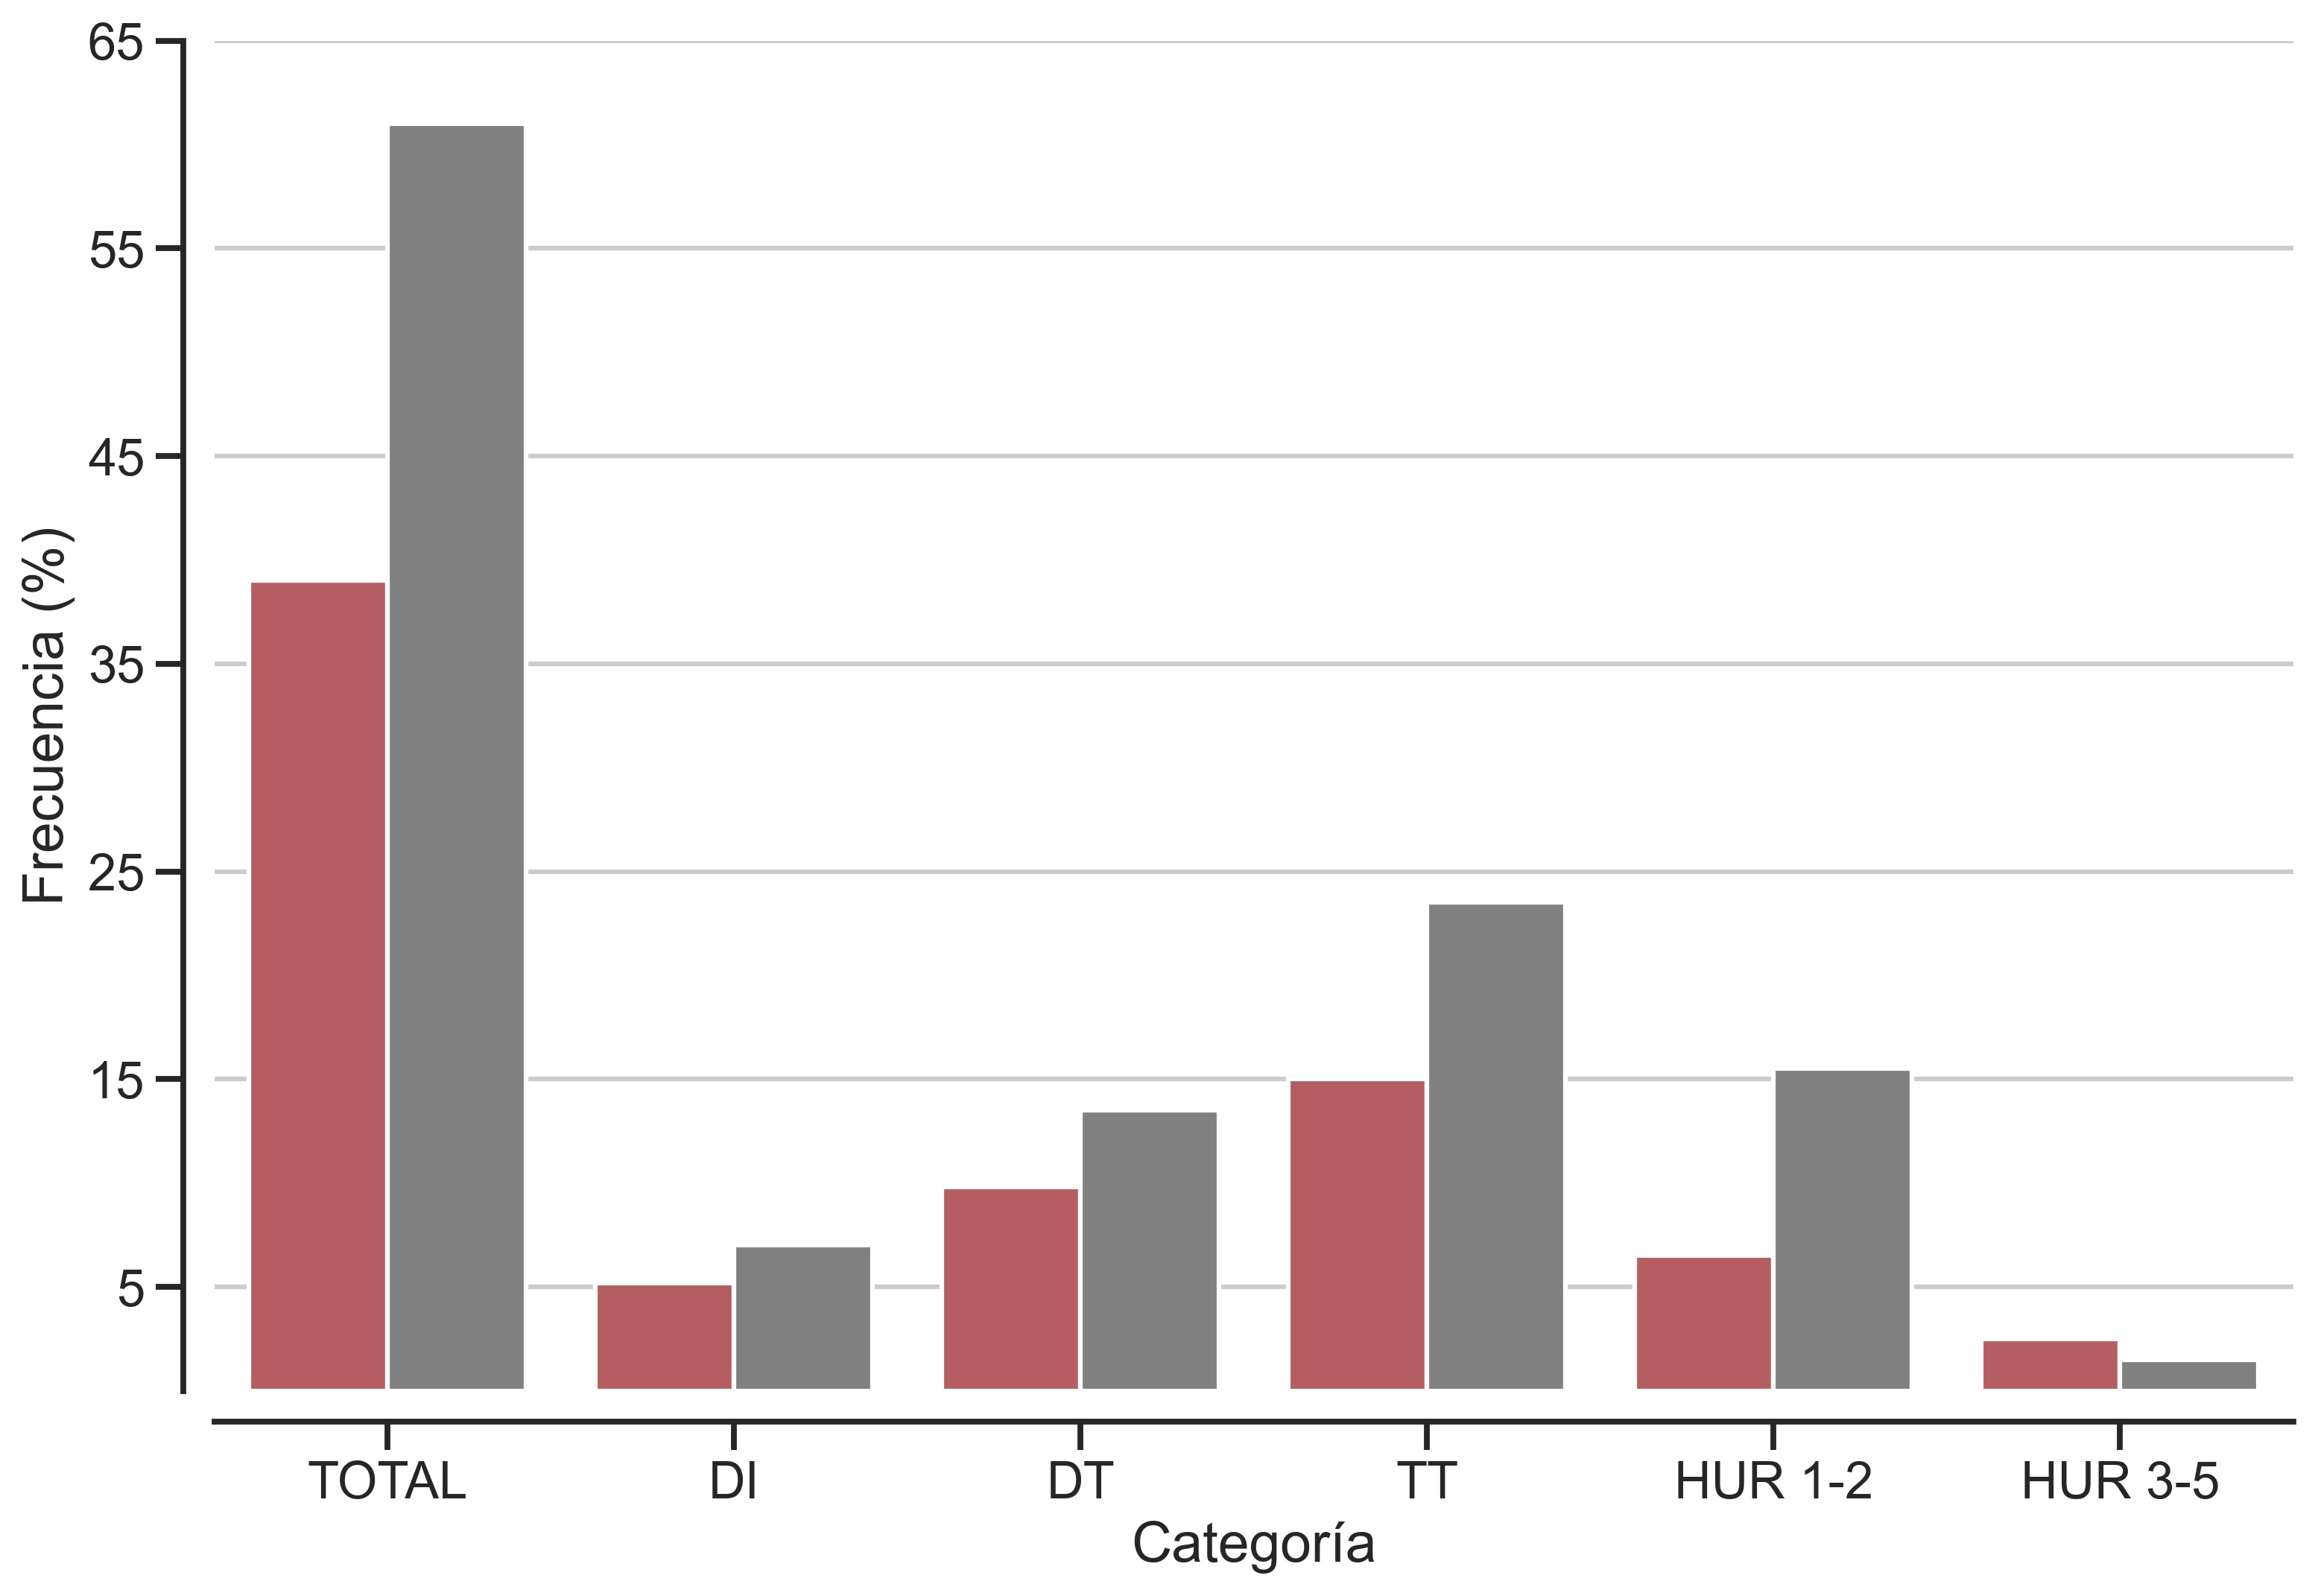
\includegraphics[scale=0.35]{Images/Figures/Fig_1_1.jpeg}
        \caption{Porcentaje de los CTs que hicieron \textit{landfalling} en las costas mexicanas. Los CTs del NA están en barras rojas  y los EP en barras grises.}
        \label{fig:fig_2}
    \end{figure}
\end{frame}

\begin{frame}{El SIAT-CT en México}
    Los desastres históricos asociados al paso de CTs en México es la principal motivación para elaborar planes de acción y mejorar la gestión integral de riesgos. En el año 2000, se propone la creación de un Sistema de Alerta Temprana de Ciclones Tropicales (SIAT-CT) como una herramienta de coordinación entre la población y Protección Civil.

    \begin{block}{Peligro por CT definido por el SIAT-CT}
    \begin{equation}
    \label{eq:1.1}
       e = \displaystyle \frac{(I+C)}{2},
    \end{equation}
    
    $e = $ Peligro \\
    $I = $ Intensidad definida por la Escala Saffir-Simpson \\
    $C = $ Escala de circulación definido por el tamaño del radio de 34 nudos
    \\~\
    \end{block}
\end{frame}

\begin{frame}
\begin{columns}
    \begin{column}{0.35\textwidth}
        \begin{block}{SIAT-CT caso TT Cristobal}
        Representación del nivel de alerta del SIAT-CT para la TT Cristóbal el 4 de junio del 2020 en sus posiciones reportadas durante las 00:00(a), 06:00(b), 12:00(c), 18:00(d) y las 00:00(e) del 5 de junio.
        \end{block}
    \end{column}
    \begin{column}{0.65\textwidth}
    \begin{figure}
        \centering
        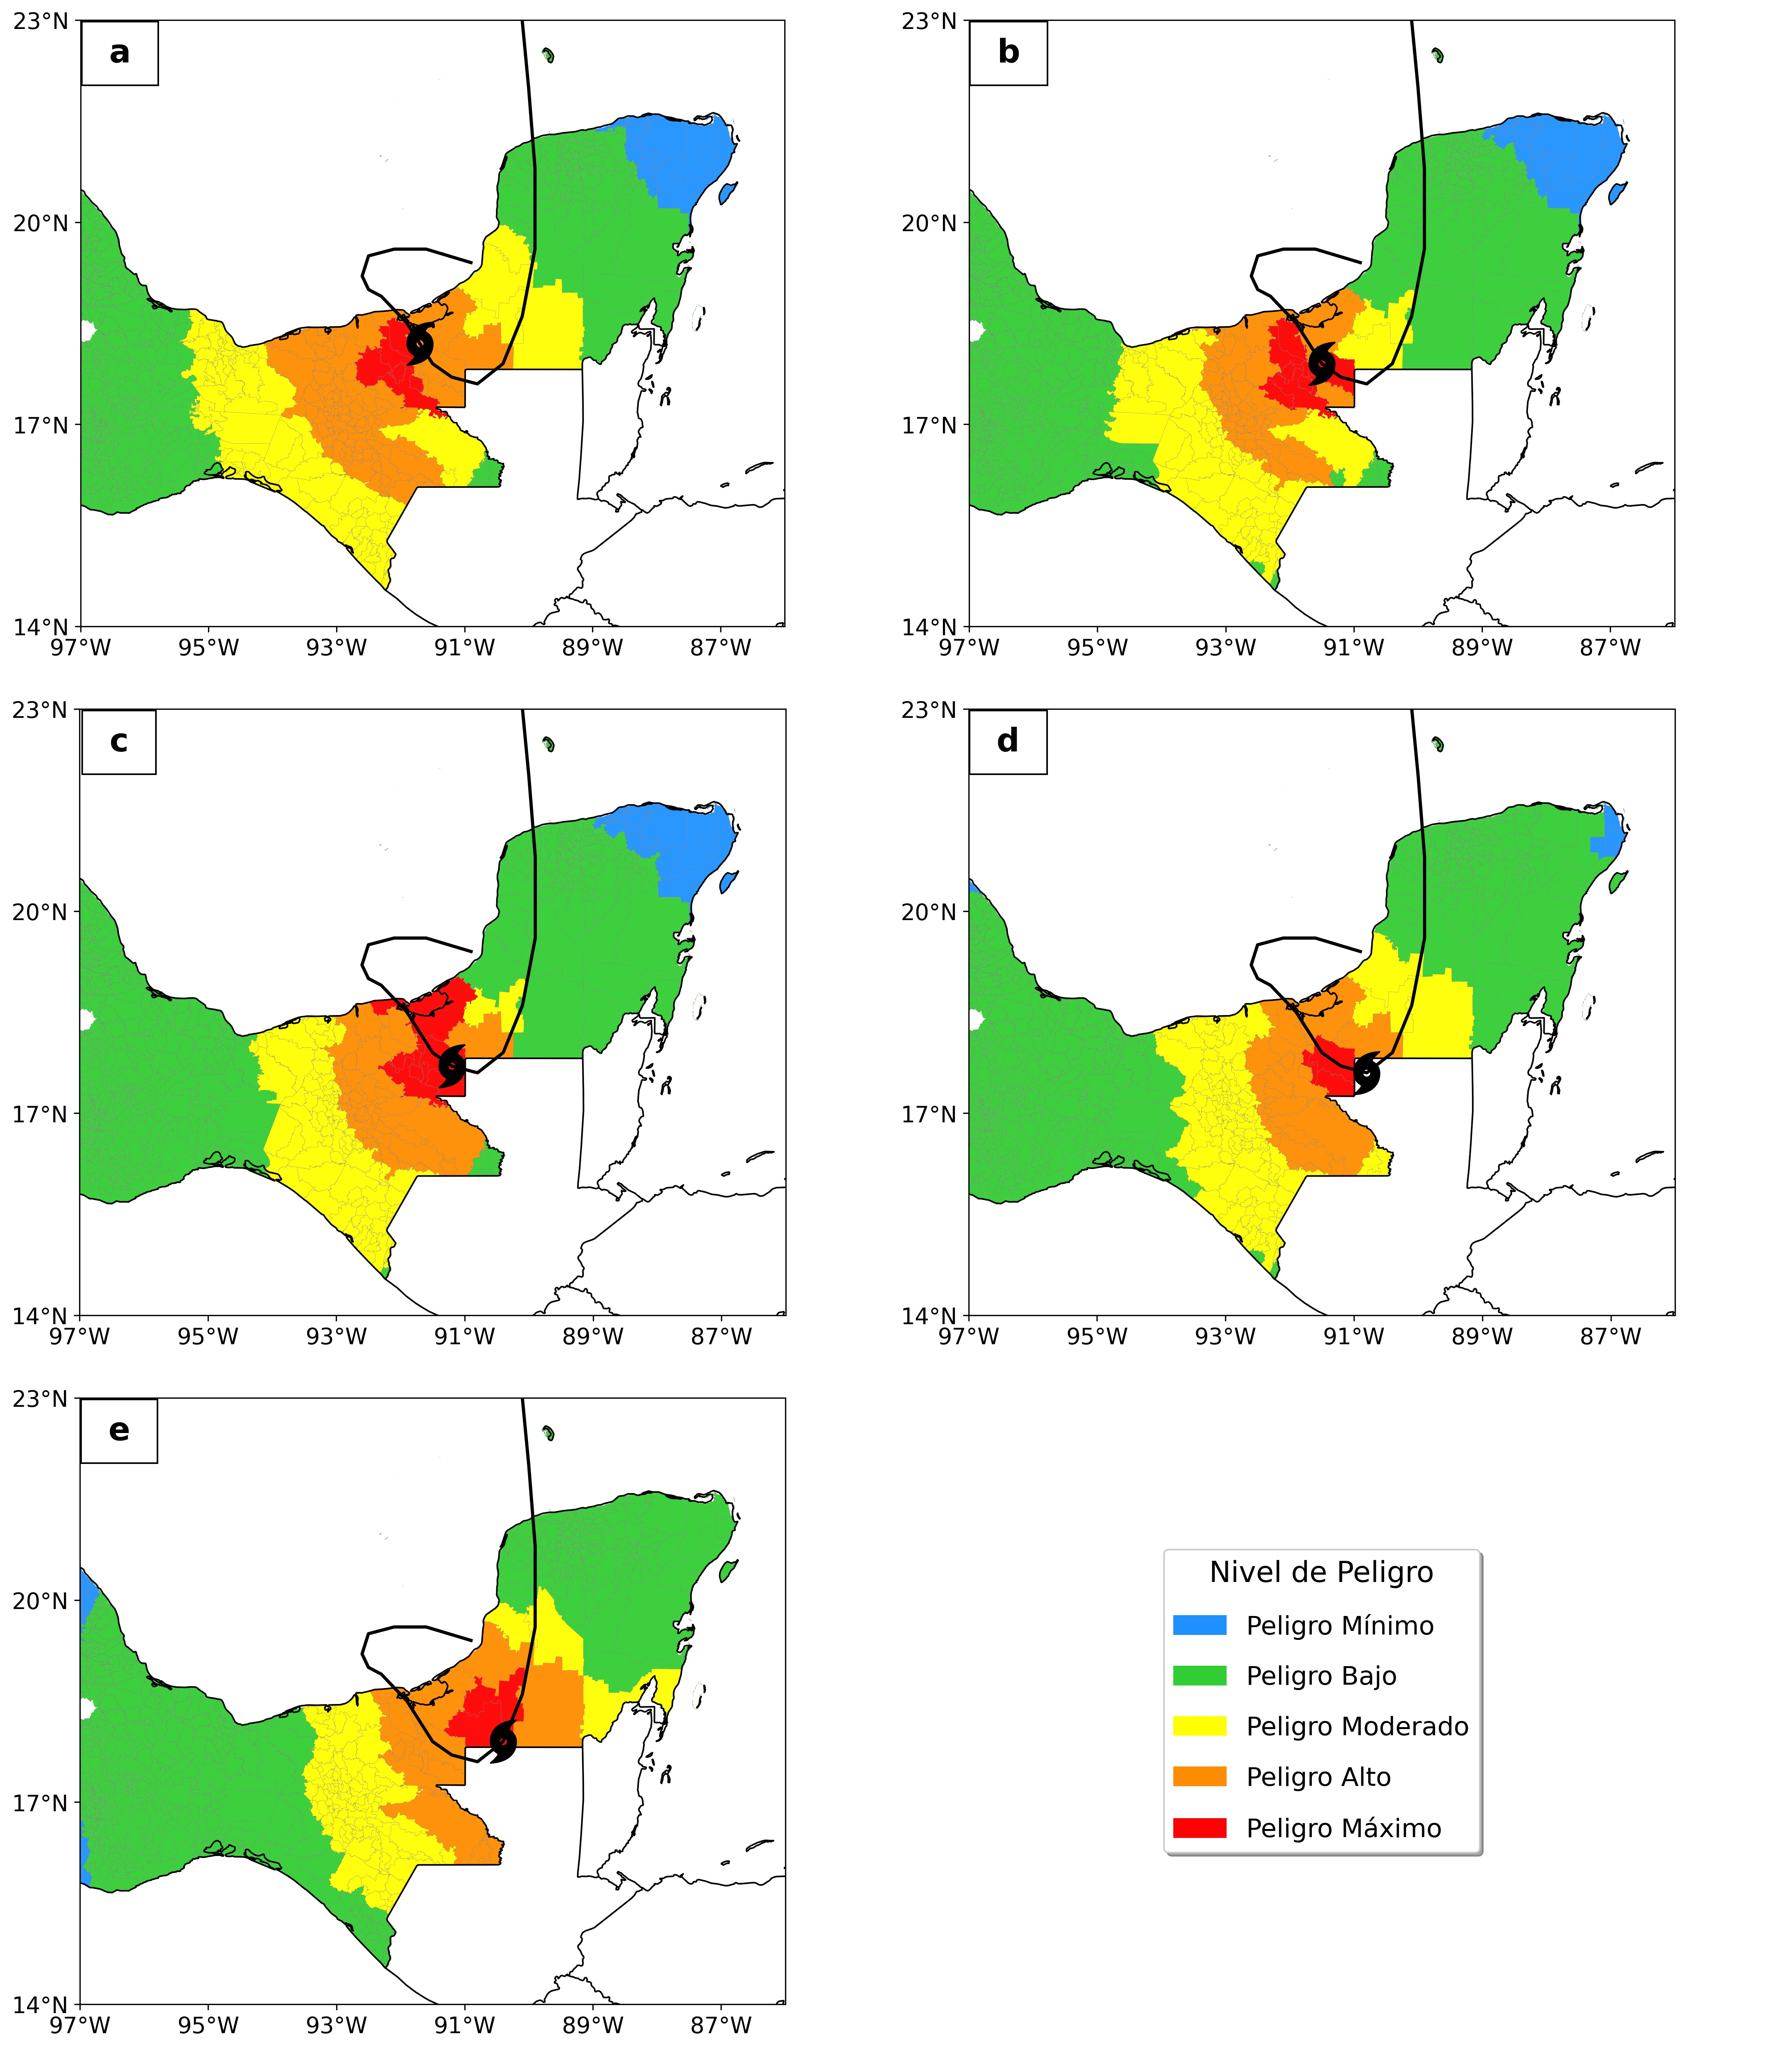
\includegraphics[scale = 0.18]{Images/Figures/Fig_1_3.jpeg}
        \label{fig:fig_3}
    \end{figure}
    \end{column}
\end{columns}
\end{frame}

\begin{frame}
    \begin{figure}
        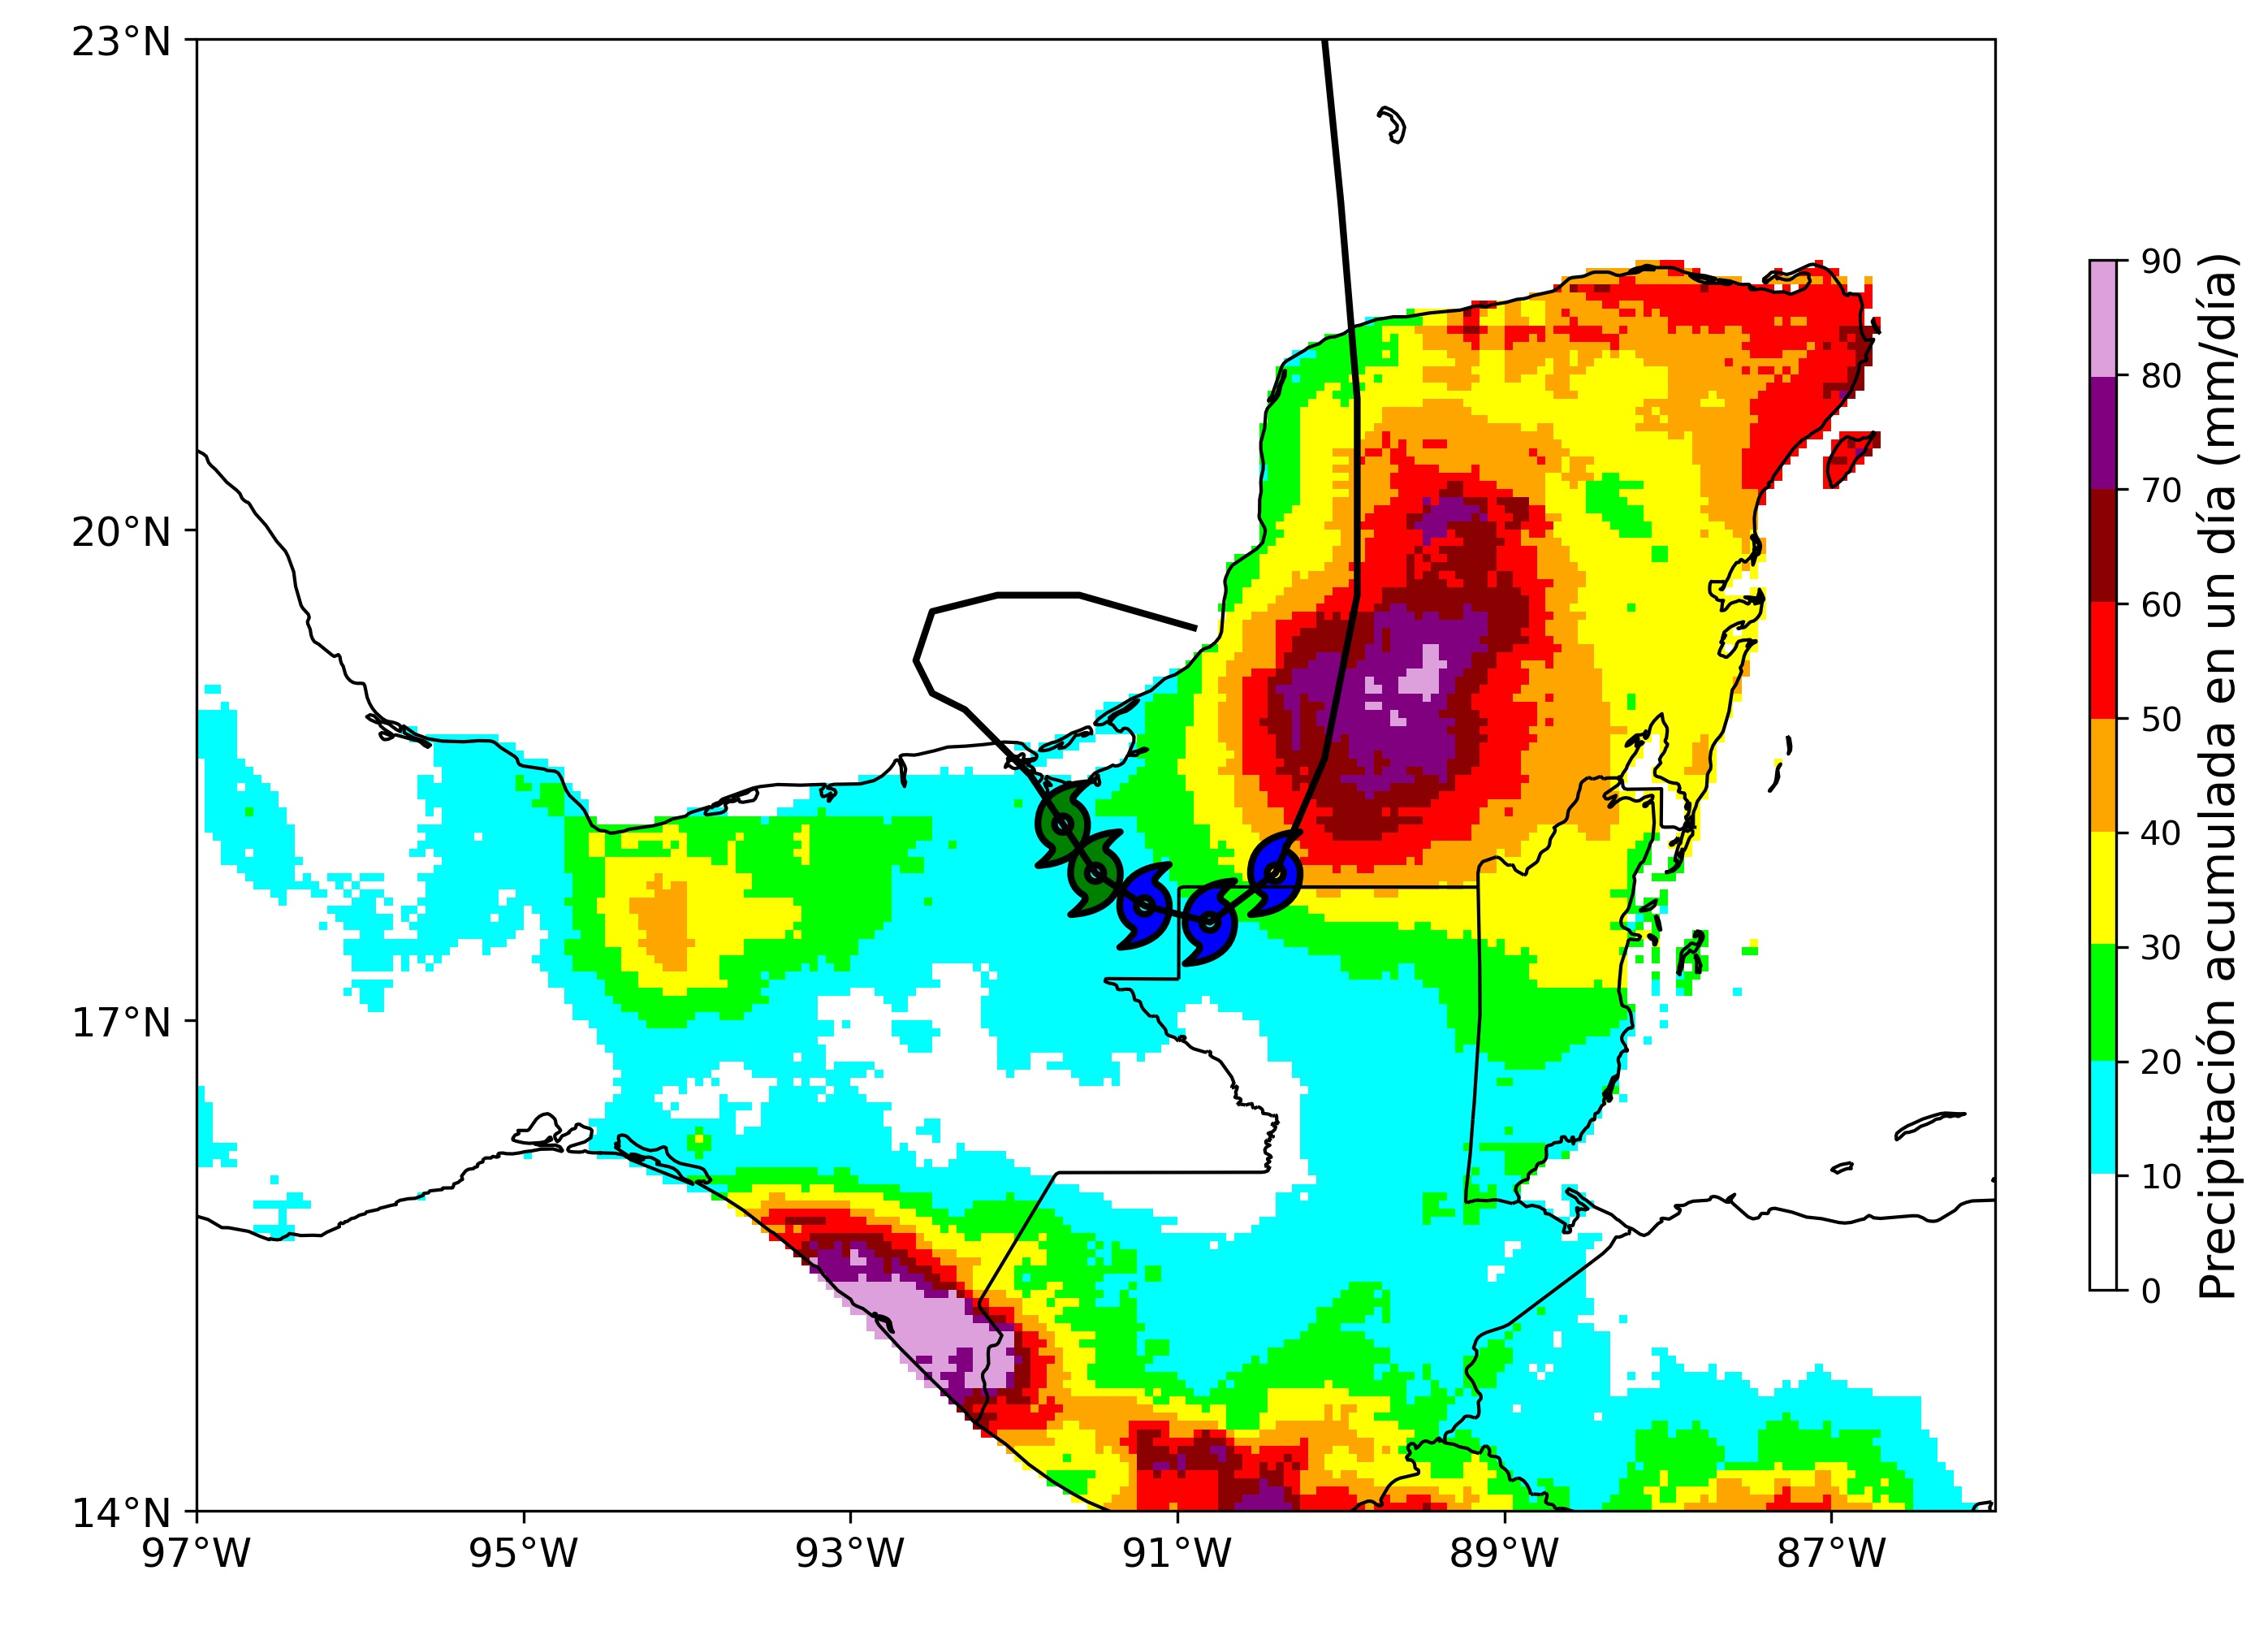
\includegraphics[scale = 0.35]{Images/Figures/Fig_1_2.jpeg}
        \caption{Valores de precipitación reportadas por CHIRPS el día 4 de junio del 2020 en el sureste de México. Las posiciones de la TT Cristóbal se muestran en verde (Tormenta Tropical) y azul (Depresión Tropical)}
        \label{fig:fig_4}  
    \end{figure}
\end{frame}

\subsection{Justificación y Objetivos}
\begin{frame}
    \hfill
    \begin{columns}
    \begin{column}{0.48\textwidth}
    \begin{block}{Justificación}
    Los estudios de CTs en México son limitados, aunque el país es impactado por la actividad ciclónica tropical cada año. Por ello, es necesario mejorar su definición de peligrosidad en el SIAT, con la finalidad de mejorar la gestión integral de riesgo. Es necesario contar con una metodología diseñada para México que defina el tamaño de los CTs.
\\~\ % Used for spacing out the block 
    \end{block}
    \end{column}
    \begin{column}{0.48\textwidth}
    \begin{block}{Objetivo General}
    Definir el tamaño de los ciclones tropicales que afectaron a México usando imágenes satelitales infrarrojas, así como analizar las relaciones estadísticas del tamaño con las variables medioambientales durante el periodo 2000-2020.
\\~\ % Used for spacing out the block 
    \end{block}
    \end{column}
    \end{columns}
\end{frame}

% \\~\ is used to force empty lines to generate to fix general typesetting within blocks.
% \\ = new line and ~\ = empty character
% \lipsum is used to generate dummy text.
